\documentclass[a4paper, 12pt]{article}

\usepackage[T2A]{fontenc}
\usepackage[utf8]{inputenc}
\usepackage[english,russian]{babel}
\usepackage[left=15mm, top=20mm, right=15mm, bottom=20mm, nohead, nofoot]{geometry}

\usepackage{hyperref}
\usepackage{graphicx}
\usepackage{wrapfig}
\usepackage{afterpage}
\usepackage{amsmath, amsfonts, amssymb, amsthm, mathtools}
\author{Хомутов Андрей, группа Б06-903}
\title{ВПВ по курсу "Электричество и магнетизм" \\ Конденсатор на высоких частотах}
\date{22 декабря 2020 г.}
%%%%%%%%%%%%%%%%%%%%%%%%%%%%%%%%%%%%%%%%%%%%%%%%%%%%%%%%%%%%%%%%%%%%%%%%%
\usepackage{graphicx, wrapfig, subcaption, setspace, booktabs}
\usepackage[protrusion=true, expansion=true]{microtype}
\usepackage[english]{babel}
\usepackage{sectsty}
\usepackage{url, lipsum}
\newcommand{\HRule}[1]{\rule{\linewidth}{#1}}
\onehalfspacing
\setcounter{tocdepth}{5}
\setcounter{secnumdepth}{5}
%%%%%%%%%%%%%%%%%%%%%%%%%%%%%%%%%%%%%%%%%%%%%%%%%%%%%%%%%%%%%%%%%%%%%%%%%


\begin{document}

\title{ \normalsize \textsc{Лабораторная работа по общей физике}
		\\ [4.0cm]
		\HRule{0.5pt} \\ [0.3cm]
		\LARGE \textbf{{Изучение рассеяния медленных электронов на атомах (эффект Рамзауэра)}}
		\HRule{0.5pt} \\ [0.1cm]
		\normalsize  \vspace*{18\baselineskip}}

\date{}

\author{Хомутов Андрей, Б06-903 \\
Рыбкина Елизавета, Б06-903 \\
ФБМФ, 2021\\ }

\maketitle
\thispagestyle{empty}
\newpage
%%%%%%%%%%%%%%%%%%%%%%%%%%%%%%%%%%%%%%%%%%%%%%%%%%%%%%%%%%%%%%%%%%%%%%%%%
\section*{Цель работы:}
Исследовать энергетическую зависимость вероятности рассеяния электронов атомами ксенона, определить энергии электронов, при которых наблюдается "просветление" ксенона, оценить размер его внешней электронной оболочки. 
%%%%%%%%%%%%%%%%%%%%%%%%%%%%%%%%%%%%%%%%%%%%%%%%%%%%%%%%%%%%%%%%%%%%%%%%%
 
\section{Теоретическая часть}
\textit{Эффективное сечение реакции} --- это величина, характеризующая вероятность перехода системы двух сталкивающихся частиц в результате их рассеяния (упругого или неупругого) в определенное конечное состояние. Сечение $\sigma$ это отношение числа таких переходов $N$ в единицу времени к плотности потока $nv$ рассеиваемых частиц, падающих на мишень, т.е. к числу частиц, падающих в единицу времени на единичную площадку, перпендикулярно к их скорости.

\begin{equation}
\sigma = \frac{N}{nv}
\end{equation}

Эффект Рамзауэра нельзя объяснить с позиции классической теории. С квантовой же точки зрения картина рассеяния выглядит следующим образом: внутри атома потенциальная энергия падающего электрона отлична от нуля, скорость электрона меняется, становясь равной $v'$ в соответствии с законом сохранения энергии 

\[E = \frac{mv^2}{2} = \frac{mv'^2}{2}+U\]

а значит, изменяется и длина его волны де-Бройля. Таким образом, по отношению к электронной волне атом ведет себя как преломляющая среда с относительным показателем преломления
\begin{equation}
n = \frac{\lambda}{\lambda'} = \sqrt{1 - \frac{U}{E}}
\end{equation}

Решение задачи о рассеянии электрона на сферическом потенциале достаточно громоздко. Поэтому рассматривают более простое одномерное приближение: электрон рассеивается на потенциальной яме конечной глубины. После решения соответствующего уравнения Шрёдингера получается выражение для коэффициента прохождения:

\begin{equation}
D = \frac{16 k_1^2 k_2^2}{16k_1^2 k_2^2 + 4\left(k_1^2-k_2^2\right)^2\sin^2\left(k_2 l\right)}
\end{equation}
где $k_1^2 = \frac{2mE}{\hbar^2}, k_2^2 = \frac{2m(E + U_0)}{\hbar^2}$.

Как легко видно, это периодическое выражение с максимумами при 

\begin{equation}
k_2 l = \pi n = \sqrt{\frac{2m(E + U_0)}{\hbar^2}}l
\end{equation}

Это же условие можно получить, рассматривая интерференцию двух волн --- прошедшей через атом и отраженной от границ атомного потенциала. Тогда получаются следующие выражения для эффективного размера атома $l$:
\begin{equation}
2l = \frac{h}{\sqrt{2m(E_1 + U_0)}}
\end{equation}

\begin{equation}
2l = \frac{3}{2}\frac{h}{\sqrt{2m(E_2 + U_0)}}
\end{equation}

Где $E_1, E_2$ --- энергии, соответствующие максимуму и минимуму прохождения электронов соответственно. Исключая $U_0$ можно найти 

\begin{equation}
l = \frac{h\sqrt{5}}{\sqrt{32m(E_2 - E_1)}}
\end{equation}


А исключая $l$ можно найти эффективную глубину потенциальной ямы атома:

\begin{equation}
U_0 = \frac{4}{5}E_2 - \frac{9}{5}E_1
\end{equation}

Так же можно вывести теоретически формулу, связывающую зависимость вероятности рассеяния электрона от его энергии:
\begin{equation}
w(V) = -\frac{1}{C} \ln \frac{I_a(V)}{I_0}
\end{equation}

С помощью неё, имея ВАХ тиратрона, можно построить график $w(V)$.

\section*{Схема установки}
Лампа-тиратрон ТГ301/1.3Б, заполненная инертным газом, расположена непосредственно на корпусе блока источников питания (БИП). Напряжение к электродам лампы подаются от источников питания, находящиеся в корпусе прибора. Регулировка напряжения и выбор режима работы установки производится при помощи ручек управления, выведенных на лицевую панель БИП.

\begin{figure}[h]
\begin{center}
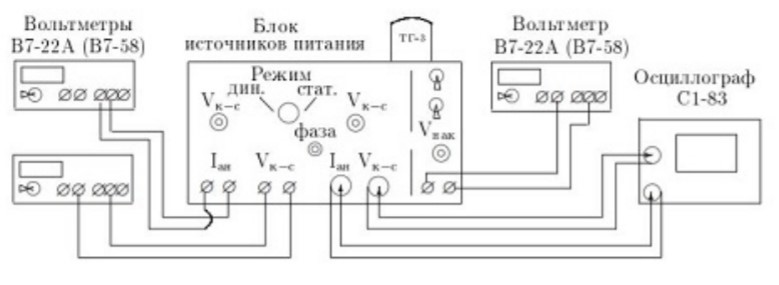
\includegraphics[width = 0.6\textwidth]{1}
\caption{Блок-схема экспериментальной установки}
\end{center}
\end{figure}

\newpage

\section{Практическая часть}
\subsection{Измерения в динамическом режиме}

\begin{table}[h!]
\begin{center}
\caption{Результаты измерения в динамическом режиме}
\begin{tabular}{|c|c|c|c|c|c|c|}
\hline
$U$, В & $E_1$, эВ & $\delta_{E_1}$, эВ & $E_2$, эВ & $\delta_{E_2}$, эВ & $V_{\text{}проб}$ & $\delta_{V_{\text{проб}}}$ \\ \hline
2,6    & 1,6       & 0,4                & 6,4       & 0,4                & 11,2              & 0,8                        \\ \hline
2,4    & 1,6       & 0,4                & 6,8       & 0,4                & 12,8              & 0,8                        \\ \hline
\end{tabular}
\end{center}
\end{table}

С помощью формул (7) и (8) рассчитаем глубину потенциальной ямы и эффиктивный размер атома:
$$
U_0 = 2.4 \pm 0.34 \text{ эВ}
$$$$
l = 307 \pm 28 \text{ пм}
$$
Также если принять $U_0 = 2.5 \text{ эВ}$, с помощью форсул (5) и (6) можно получить:
$$
l_1 = 303 \pm 19 \text{ пм}
$$$$
l_2 = 305 \pm 9 \text{ пм}
$$

Пробой происходит в среднем при $V = 12,0 \pm 0,4 \text{ В}$б поэтому можно предположить что исследуемый газ - ксенон (потенциал ионизации составляет 12.1 эВ).

\subsection{Измерения в статическом режиме}


Построим полученный ВАХ на графике (рис.2). Проводя аналогичные расчеты:
$$
U_0 = 1.78 \pm 0.06 \text{ эВ}
$$$$
l = 316 \pm 5 \text{ пм}
$$

Из формулы (4) получим что слудющие максимумы соотвествуют напряжениям $E_2 \simeq 20 \text{ эВ, }E_3 \simeq 48 \text{ эВ}$. Но при данном потенциале ионизации их невозможно увидеть.

Также с помощью формулы (9) построим график вероятности рассеяния $w(V)$ (рис. 3).

\newpage

\begin{figure}[h!] %% ШАБЛОН ДЛЯ ДВУХ КАРТИНОК
\begin{center}
\begin{minipage}[h]{0.49\linewidth}
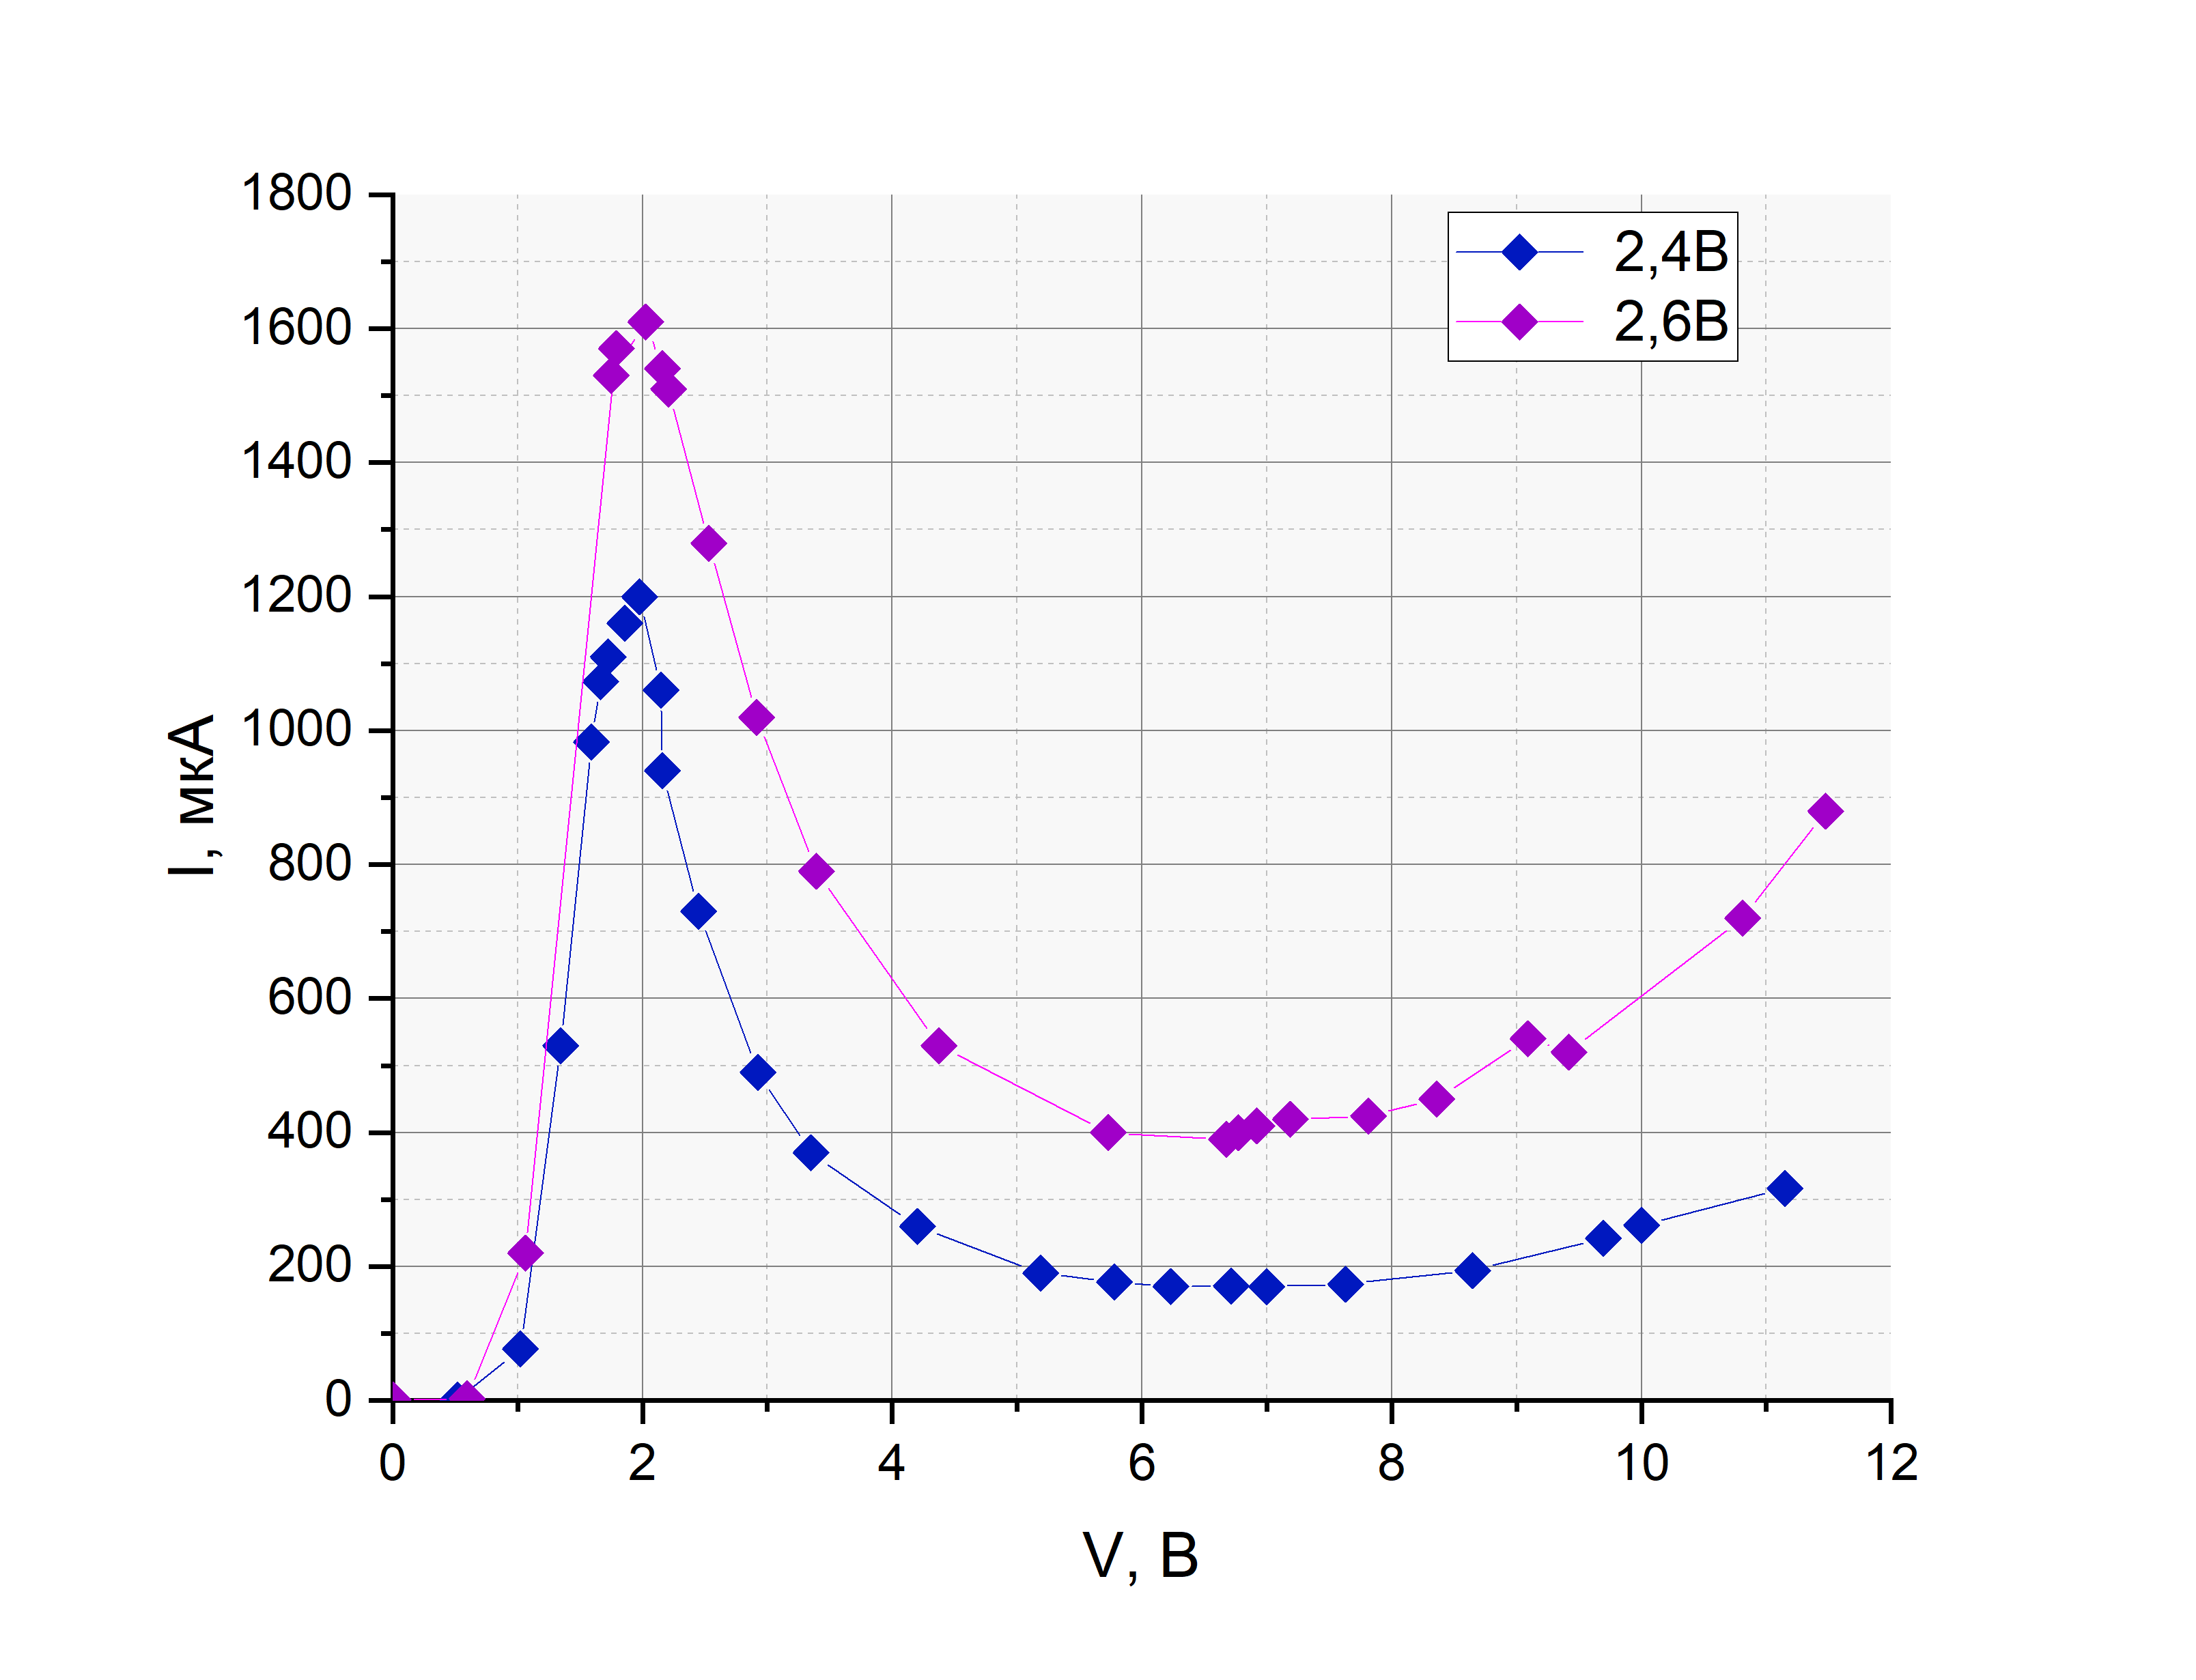
\includegraphics[width=1\linewidth]{Рамзауэр.PNG}
\caption{ВАХ тиратрона в статическом режиме} %% подпись к рисунку
\label{ris:experimoriginal} %% метка рисунка для ссылки на него
\end{minipage}
\hfill 
\begin{minipage}[h]{0.49\linewidth}
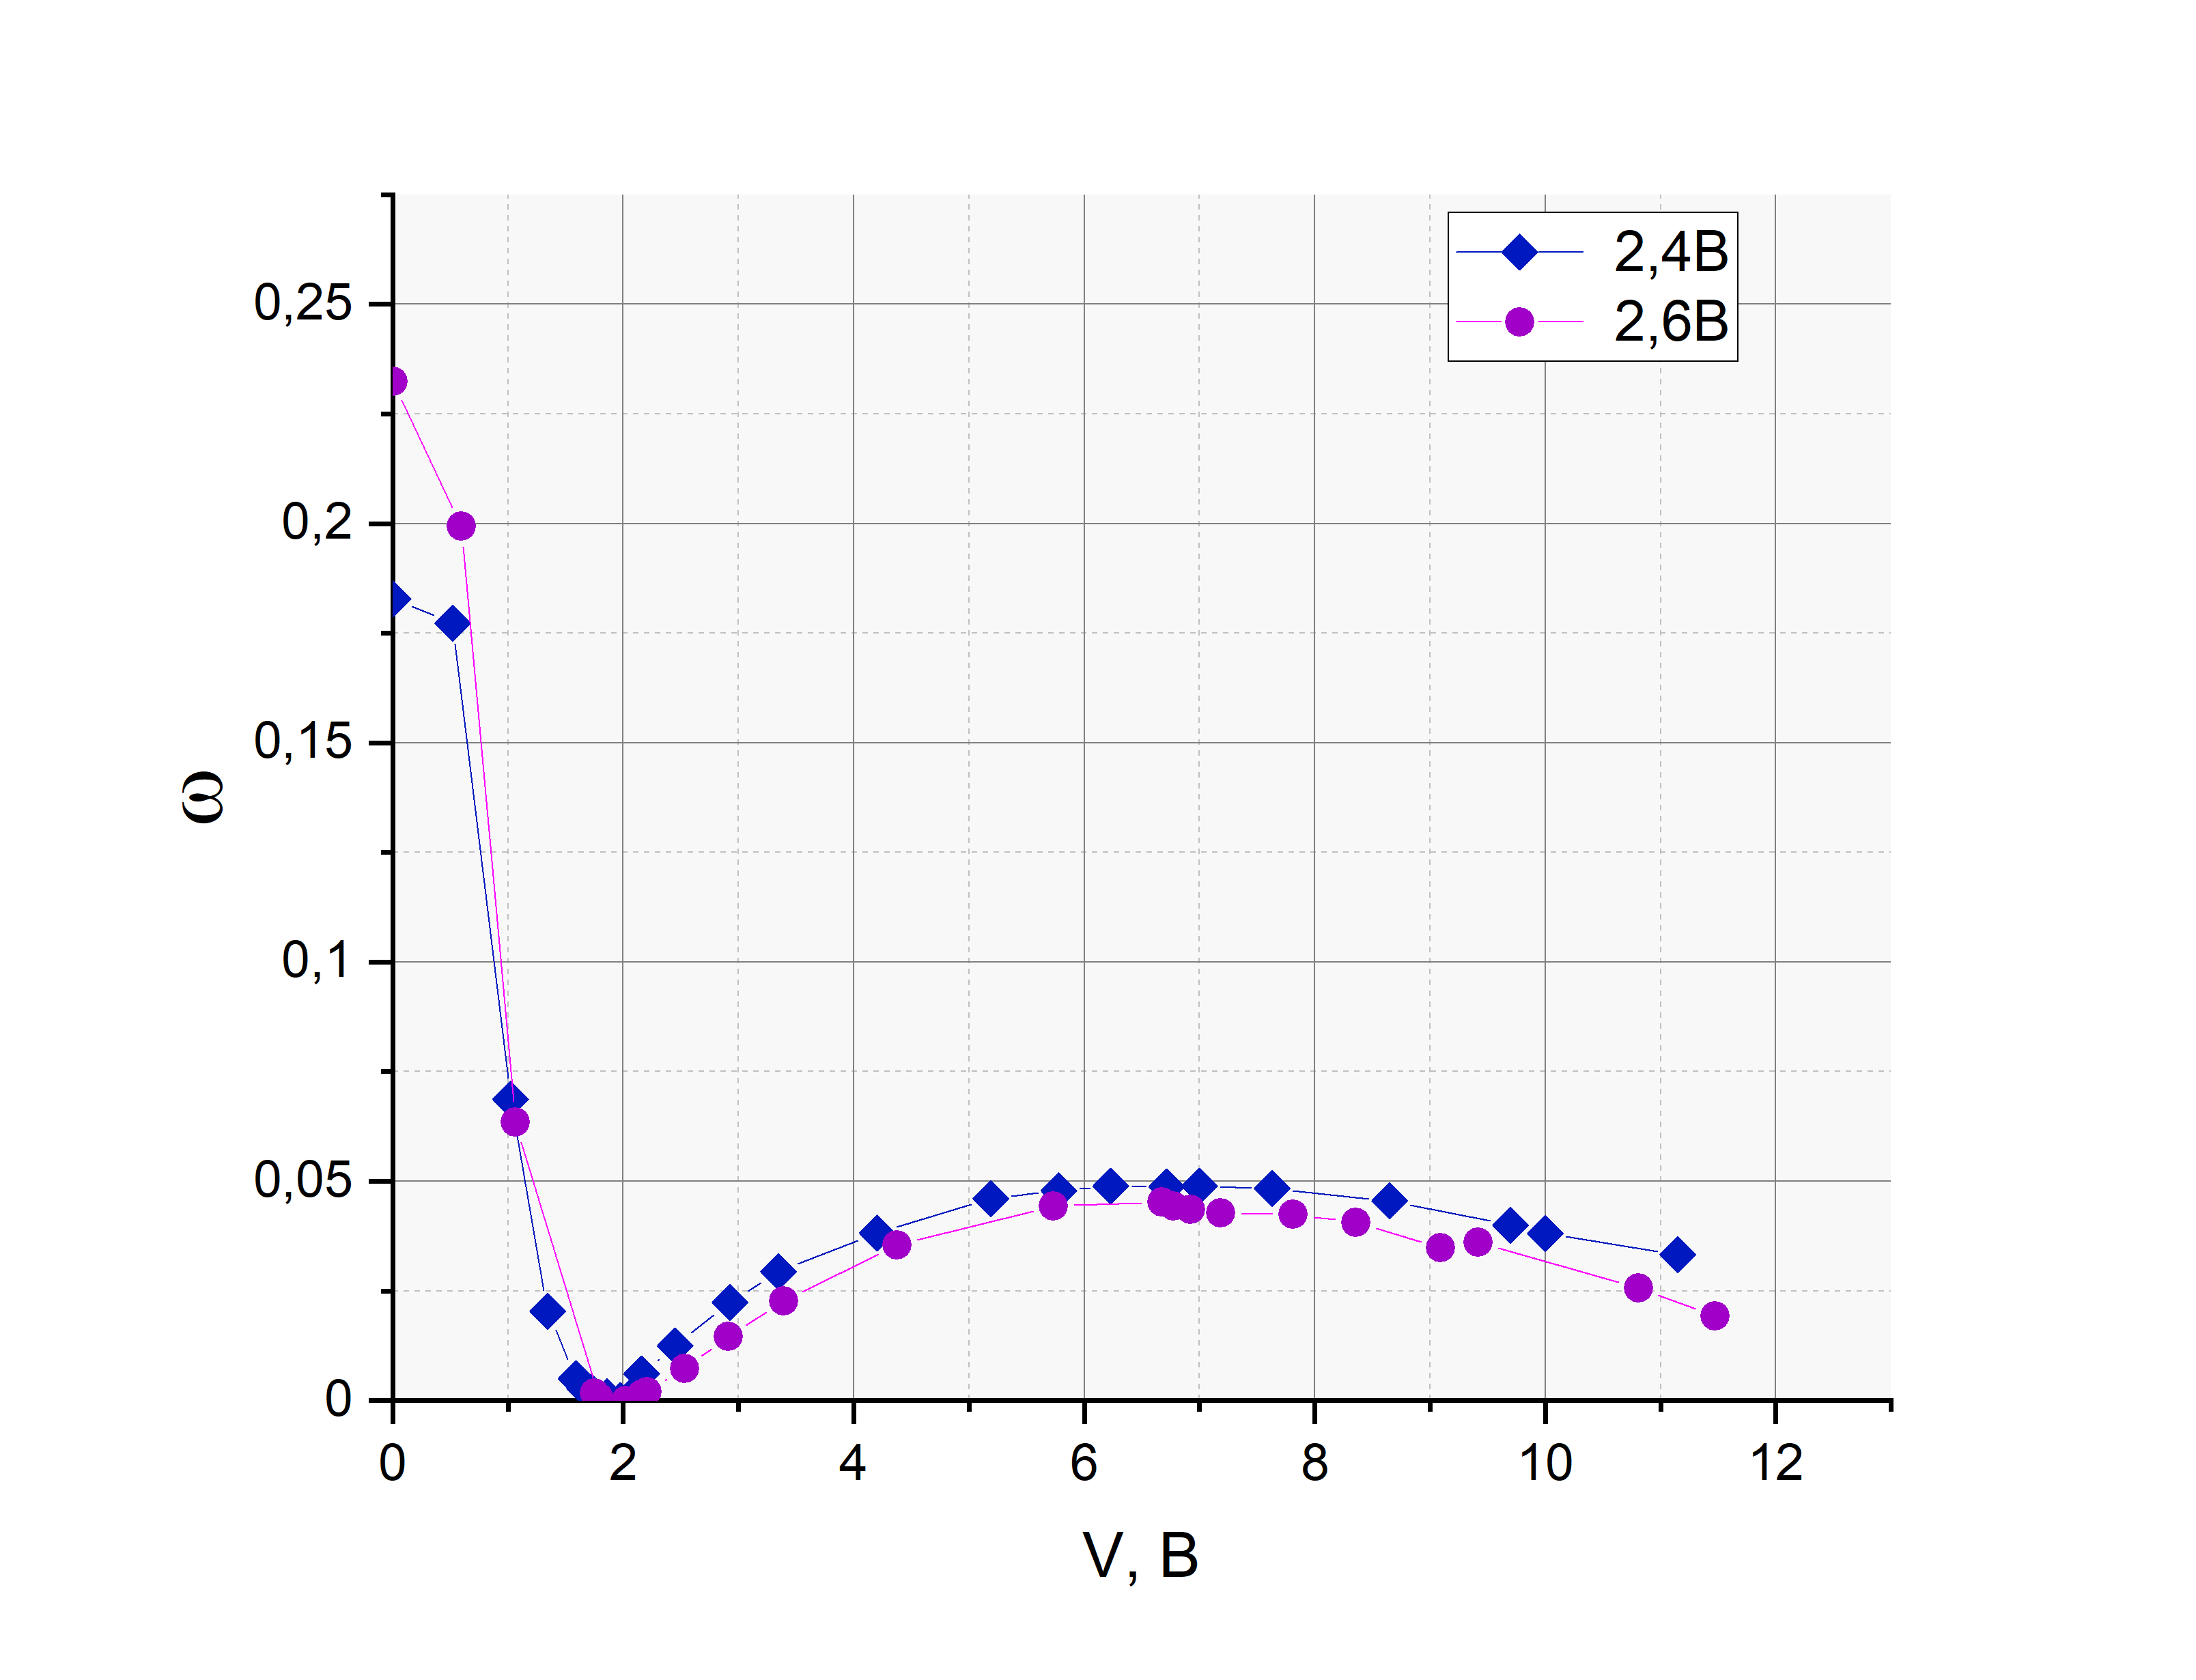
\includegraphics[width=1\linewidth]{w.PNG}
\caption{Зависимость вероятности рассеяния от напряжения}
\label{ris:experimcoded}
\end{minipage}
\end{center}
\end{figure}





%%%%%%%%%%%%%%%%%%%%%%%%%%%%%%%%%%%%%%%%%%%%%%%%%%%%%%%%%%%%%%%%%%%%%%%%%
 \section{Выводы}
В этой лабораторной работы мы могли пронаблюдать ВАХ тиратрона в динамическом и статическом режимах измерения. Путем снятия точек в статическом режиме был построен график, согласующийся с теорией, по которому можно было определить максимум и минимум тока и соответствующие им напряжения. Для динамического режима измерения напряжения были сняты по осцилограмме. С помощью этих величин было возможно определить глубину потенциальной ямы $U_0$, при этом расчет по данным динамического измерения, дал лучший результат и был довольно близок к справочным 2,5 В. Оба метода хорошо себя зарекомендовали в определении размера электронной оболочки $l$, давая приблизительно одинаковые результаты около 300 пм (справочные данные для ковалентного радиуса ксенона ~ 140 пм). Наконец, был построен график $w(V)$, соответствующий ожидаемому виду.
\newpage
\section{Приложения}

\begin{table}[h!]
\begin{center}
\caption{Результаты измерения в статическом режиме}
\begin{tabular}{|c|c|c|c|c|}
\hline
\multirow{}{}{} & \multicolumn{4}{c|}{Напряжение накала}                  \\ \cline{2-5} 
                  & \multicolumn{2}{c|}{2,4 В} & \multicolumn{2}{c|}{2,6 В} \\ \hline
№                 & $V$, В      & $I$, мкА     & $V$, В      & $I$, мкА     \\ \hline
1                 & 0,004       & 0,8          & 0,004       & 1,1          \\ \hline
2                 & 0,52        & 1            & 0,595       & 3,1          \\ \hline
3                 & 1,023       & 76,7         & 1,063       & 220          \\ \hline
4                 & 1,345       & 530          & 1,79        & 1570         \\ \hline
5                 & 1,59        & 983          & 1,75        & 1530         \\ \hline
6                 & 1,665       & 1073         & 2,026       & 1610         \\ \hline
7                 & 1,725       & 1110         & 2,16        & 1540         \\ \hline
8                 & 1,86        & 1160         & 2,209       & 1510         \\ \hline
9                 & 1,977       & 1200         & 2,533       & 1280         \\ \hline
10                & 2,15        & 1060         & 2,915       & 1020         \\ \hline
11                & 2,16        & 940          & 3,393       & 790          \\ \hline
12                & 2,45        & 730          & 4,374       & 530          \\ \hline
13                & 2,926       & 490          & 5,73        & 400          \\ \hline
14                & 3,348       & 370          & 6,677       & 390          \\ \hline
15                & 4,202       & 260          & 6,773       & 400          \\ \hline
16                & 5,19        & 190          & 6,921       & 410          \\ \hline
17                & 5,78        & 177          & 7,187       & 420          \\ \hline
18                & 6,23        & 170          & 7,815       & 425          \\ \hline
19                & 6,715       & 171          & 8,36        & 450          \\ \hline
20                & 7           & 170          & 9,092       & 540          \\ \hline
21                & 7,63        & 173,7        & 9,42        & 520          \\ \hline
22                & 8,648       & 194          & 10,812      & 720          \\ \hline
23                & 9,696       & 242          & 11,475      & 880          \\ \hline
24                & 10          & 262          &             &              \\ \hline
25                & 11,15       & 317          &             &              \\ \hline
\end{tabular}
\end{center}
\end{table}

\begin{figure}[h!]
    \begin{center}
    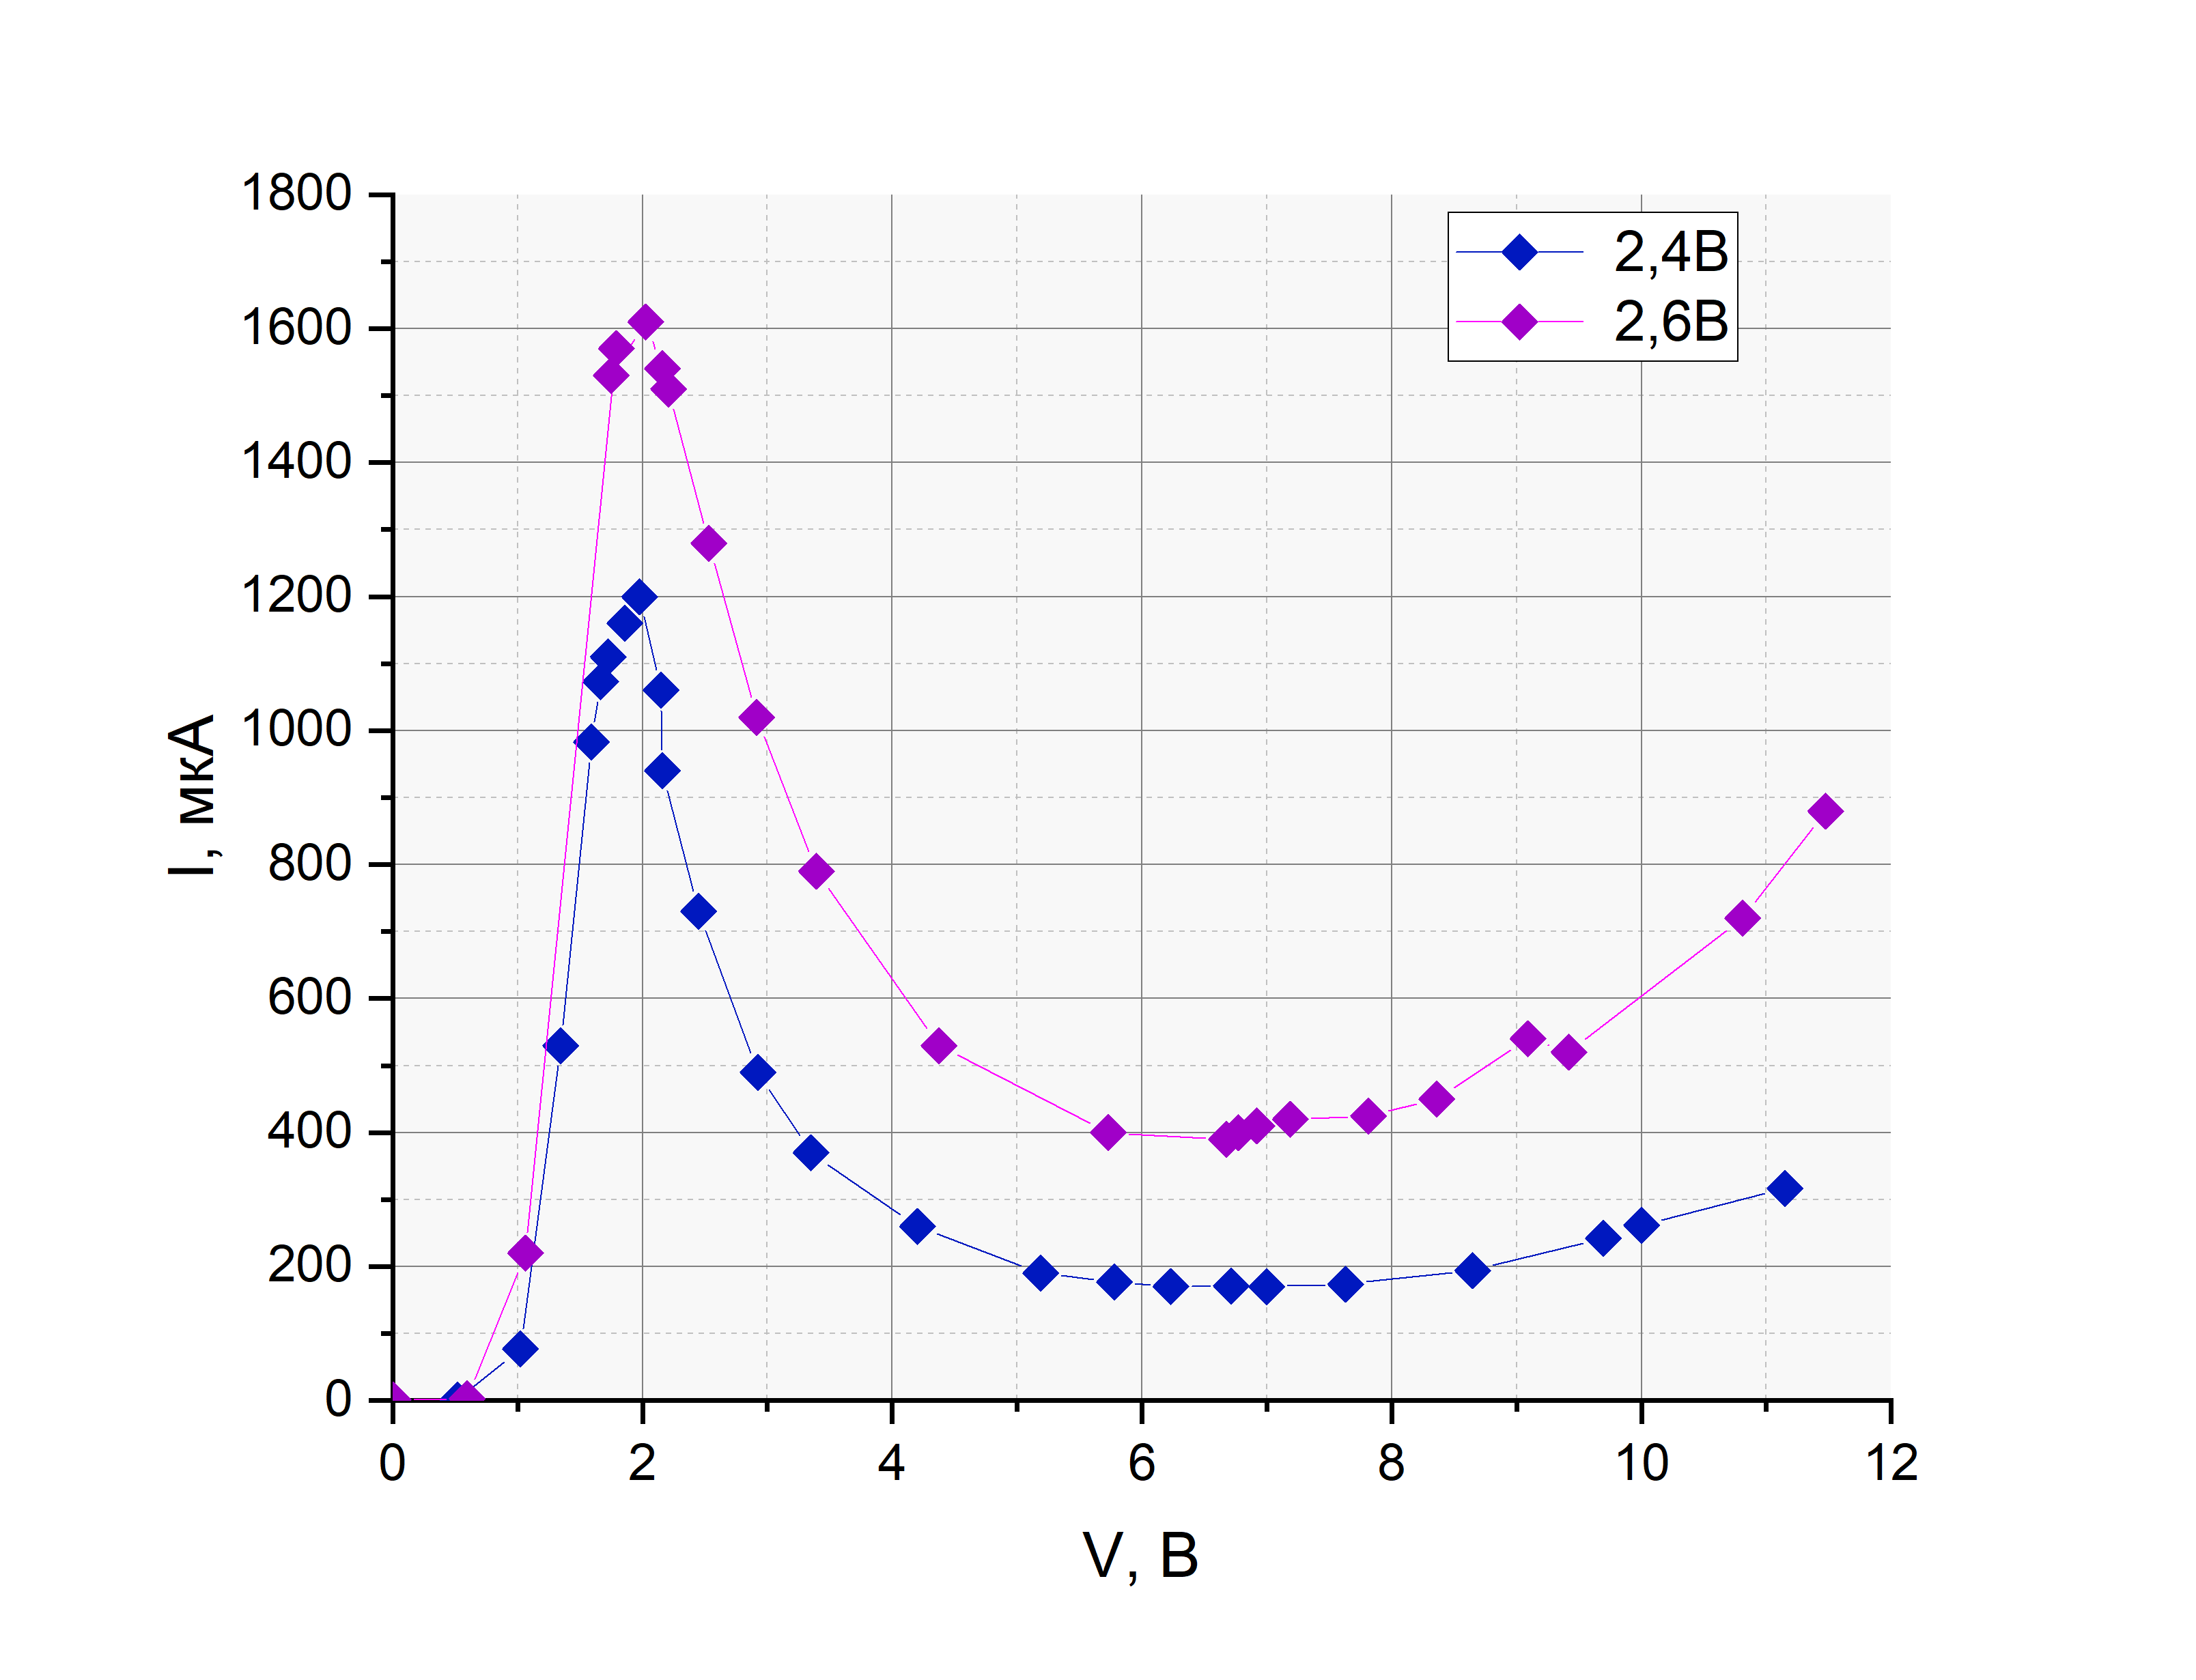
\includegraphics[width=0.99\textwidth]{Рамзауэр.png}
    \end{center}
    \caption{ВАХ тиратрона в статическом режиме}
\end{figure}
\begin{figure}[h!]
    \begin{center}
    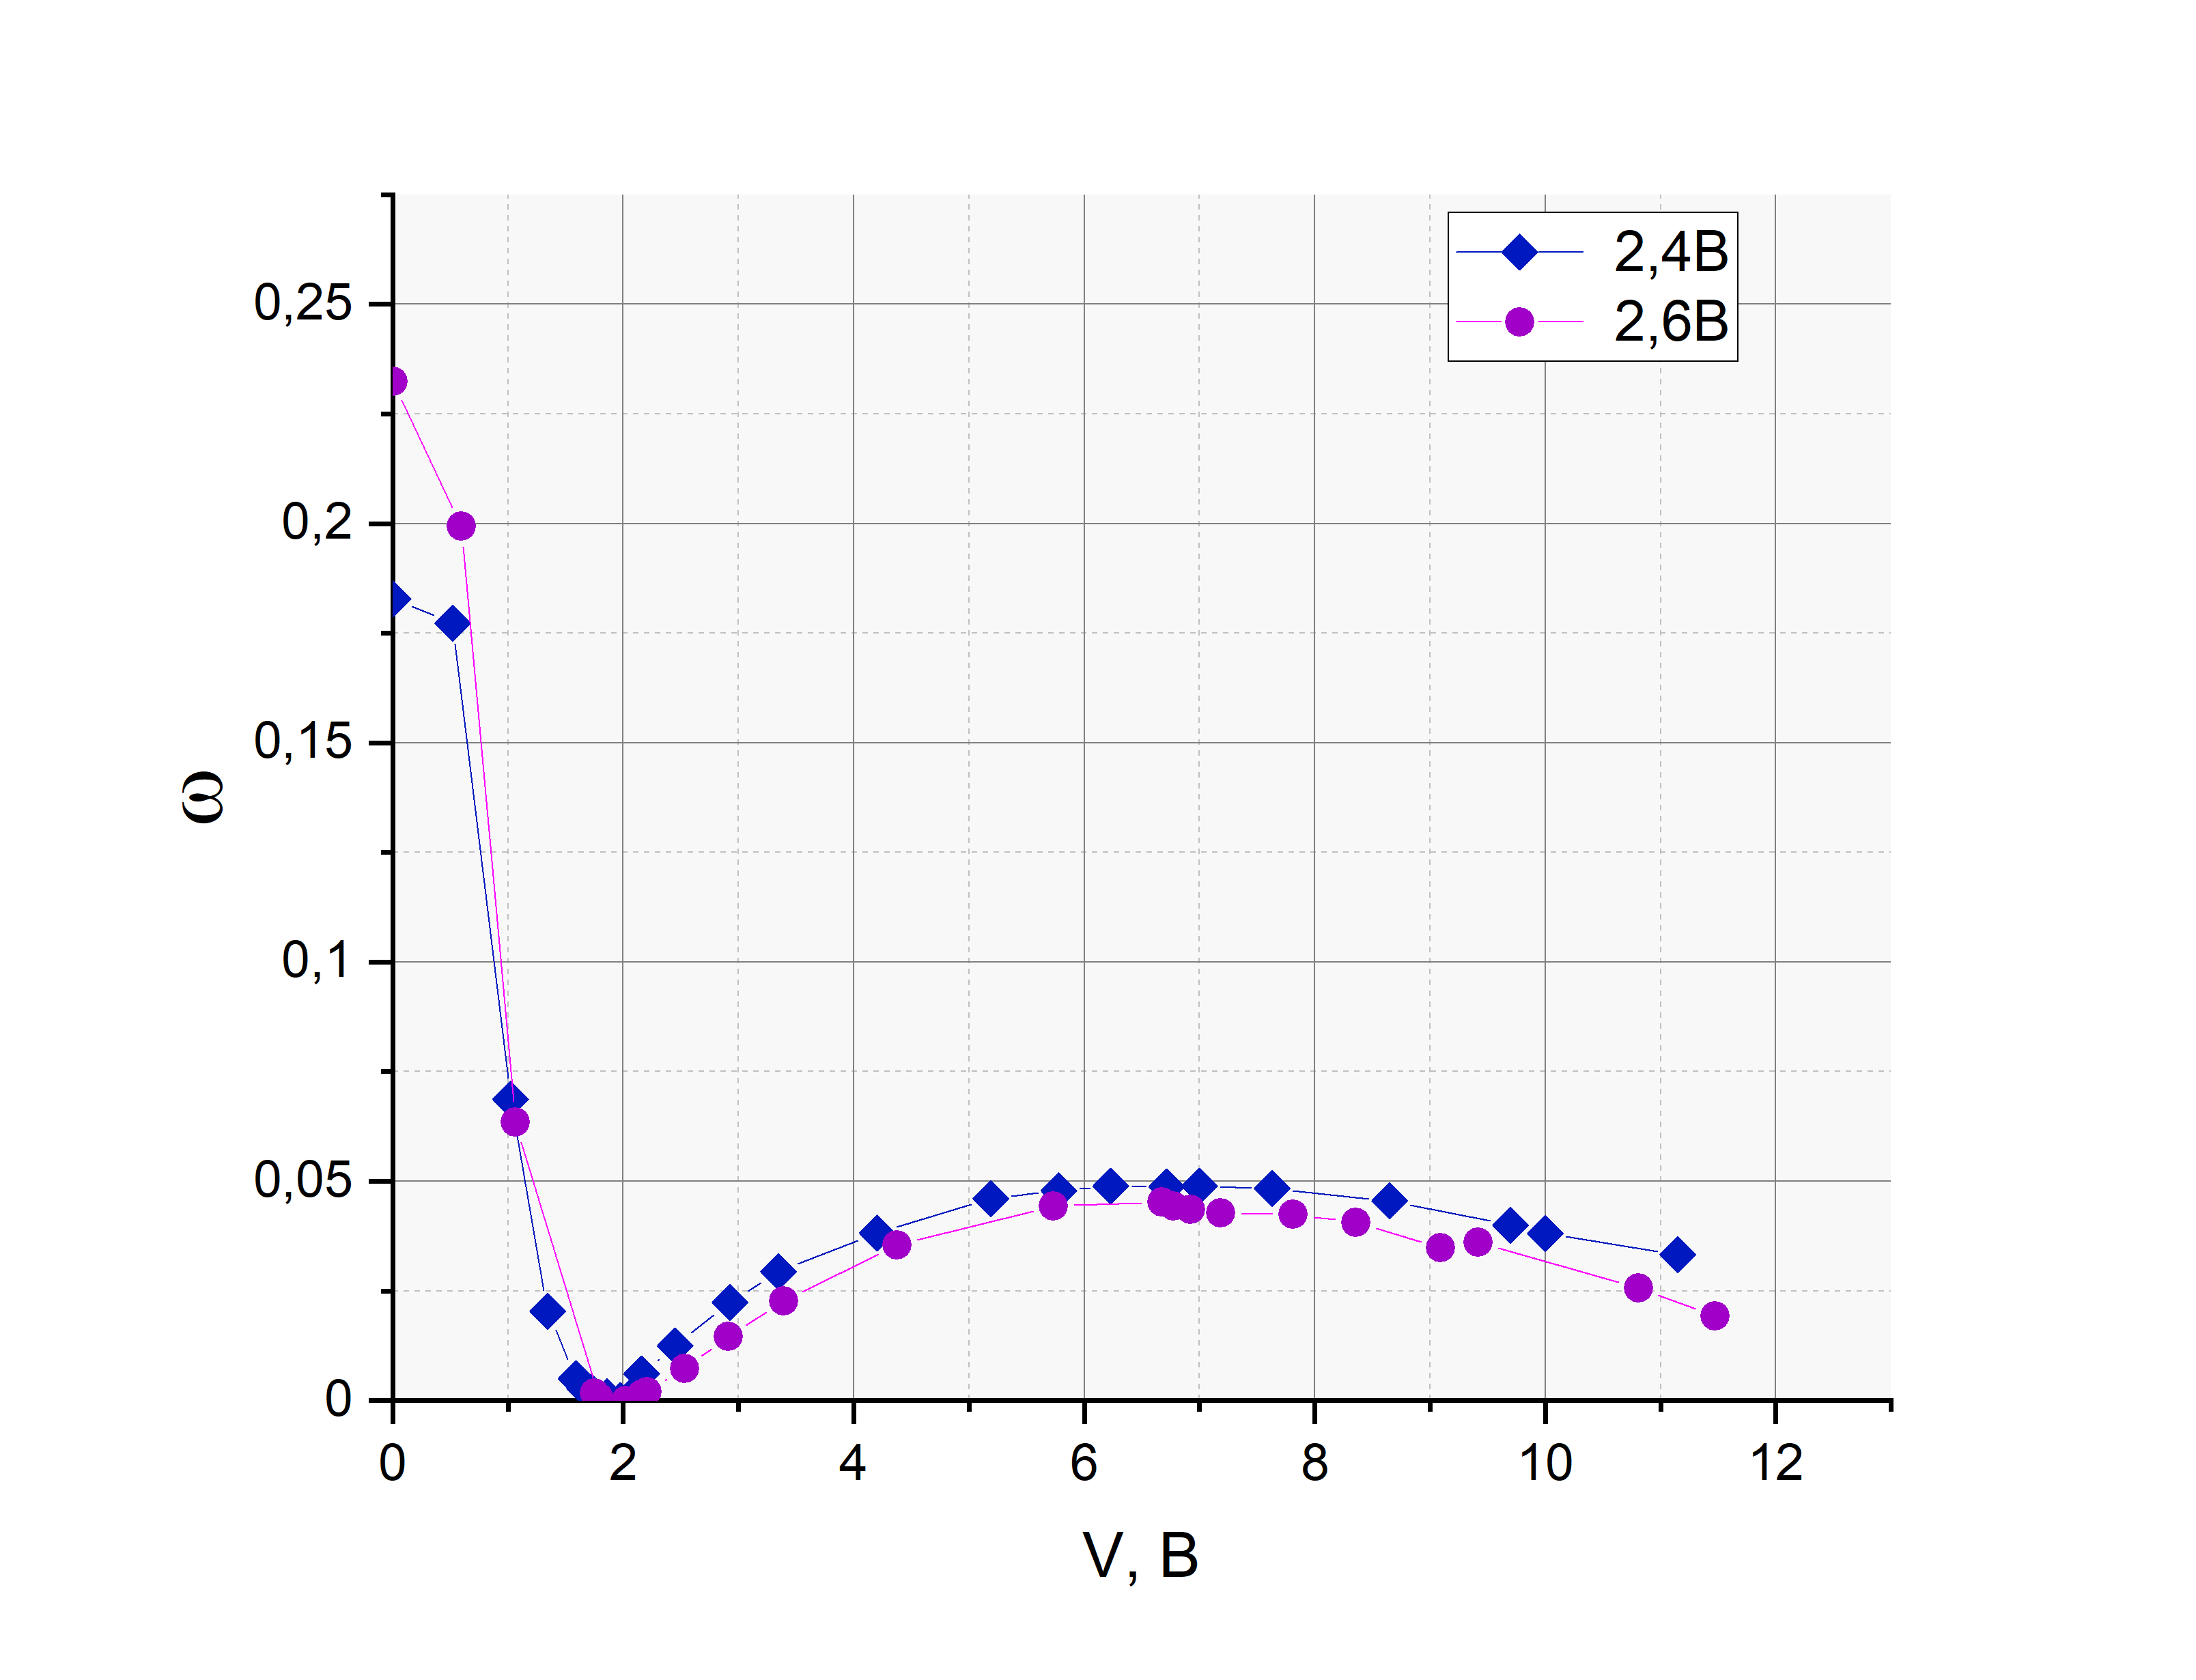
\includegraphics[width=0.99\textwidth]{w.png}
    \end{center}
    \caption{Зависимость вероятности рассеяния от напряжения}
\end{figure}

$$
n_j = \sum_{i=1}^{N} I(seq_i(date) \in dates\_interval_j)
$$

$$
n\_prot\_muts_j = \frac{\sum_{i=1}^{N} seq_i(q\_prot\_muts)I(seq_i(date) \in dates\_interval_j)}{\sum_{i=1}^{N} I(seq_i(date) \in dates\_interval_j)}
$$

$$
n\_prot\_muts_j = \frac{\sum_{i=1}^{N} seq_i(q\_prot\_muts)I(seq_i(clade) = clade_j)}{\sum_{i=1}^{N}I(seq_i(clade) = clade_j)}
$$

$$
std_j = \frac{\sum_{i=1}^{N} seq_i(prot_k\_loc\_std)I(seq_i(clade) = clade_j)}{\sum_{i=1}^{N}I(seq_i(clade) = clade_j)}
$$

$$
std_k = \frac{\sum_{i=1}^{N} seq_i(prot_k\_loc\_std)I(seq_i(clade) = GRA)I(seq_i(date) \in Jul2022)}{\sum_{i=1}^{N}I(seq_i(clade) = GRA)I(seq_i(date) \in Jul2022)}
$$
$$
std_k\_norm = \frac{\sum_{i=1}^{N} \frac{seq_i(prot_k\_loc\_std)}{len(prot_k)}I(seq_i(clade) = GRA)I(seq_i(date) \in Jul2022)}{\sum_{i=1}^{N}I(seq_i(clade) = GRA)I(seq_i(date) \in Jul2022)}
$$
\end{document}

















\begin{table}[h!]
\begin{center}
\caption{...}
\begin{tabular}{|c|c|c|c|c|}

\end{tabular}
\end{center}
\end{table}


\begin{figure}[h!]
    \begin{center}
    \includegraphics[width=0.8\textwidth]{xxx.png}
    \end{center}
    \caption{...}
\end{figure}

\begin{figure}[h!] %% ШАБЛОН ДЛЯ ДВУХ КАРТИНОК
\begin{center}
\begin{minipage}[h]{0.40\linewidth}
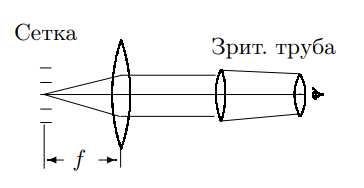
\includegraphics[width=1\linewidth]{plus_lens.PNG}
\caption{...} %% подпись к рисунку
\label{ris:experimoriginal} %% метка рисунка для ссылки на него
\end{minipage}
\hfill 
\begin{minipage}[h]{0.40\linewidth}
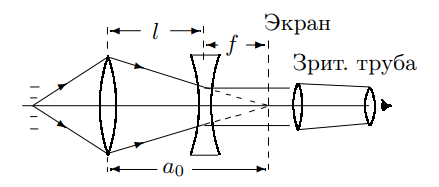
\includegraphics[width=1\linewidth]{minus_lens.PNG}
\caption{..}
\label{ris:experimcoded}
\end{minipage}
\end{center}
\end{figure}

\subsection{...}
\subsubsection{...}



\subsubsection{...}